\chapter{The Standard Model of Particle Physics}
\label{chapter:SM}


\epigraph{\textit{Ex pede Herculem. \newline(From the feet, Hercules.)}}{--Herodotus, Book IV, Section LXXXII. Plutarch}

%TODO measured eighteen parameters catalog

The Standard Model of Particle Physics (SM) is the epitome of human understanding of physical elementary building blocks to date. From the SM, the properties and interactions of seventeen fundamental particles and their interactions are laid out. It provides the foundational understanding of matter and its interactions on the quantum scale.

This chapter provides an overview of the SM: In Section~\ref{sec:SM}, a theoretical description of the SM is given, the mechanism of the theory is discussed, and the Gauge fields and their particles are listed. As a complete picture of the SM relies on experimental measurements of its parameters, the measured values of the eighteen parameters are also cataloged in this section. Despite the many advances made by the SM, there remain many open
questions left to be solved. Some of them are motivators to studies performed in this thesis. In Section~\ref{sec:UnresolvedSM}, a summarized list of resolved problems to the SM is presented.

\section{Standard Model: Theoretical Description}
\label{sec:SM}

Mathematically, the SM is a gauge theory under the 
Quantum Field Theory (QFT) framework. Particles are represented as different quantized fields operators. The particle interactions are described by the SM Lagrangian which takes the form as shown in Eqaution~\ref{eq:SMLagrangian}. Through the SM Lagrangian, all physics laws concerning the particle interaction channels, their interaction cross sections and their motion through scattering can be derived.

\subsection{Symmetry}
Symmetry is the cornerstone of many laws in physics. Mathematically, it's the invariance of quantities through transformation, and is shown by the Noether's Theorem~\cite{sarlet1981generalizations} to be related to conservation laws in physics:

    \begin{itemize}
        \item Spatial Translational Symmetry $\leftrightarrow$ Translational Momentum Conservation
        \item Time Symmetry $\leftrightarrow$ Energy Conservation
        \item Rotational Symmetry $\leftrightarrow$ Angular Momentum Conservation
    \end{itemize}

    A symmetry and its transformation can be summarized by the mathematical language of group theory. In group theory, continuous transformation is described by the Lie group and the discrete transformation is represented by a finite group. 

    There are two kinds of symmetries in the SM, external symmetries and internal symmetries. External symmetries are related to space-time transformation of the particle; internal particle symmetries are related to other particle properties other than space-time. 

\subsubsection{External Symmetries} 
External symmetries are transformations on the space-time coordinates, The SM external symmetries can be summarized by the following three groups, known collectively as the \textit{Poincar\'{e} group}. Each of the terms conserves a physics quantity. 
    
     \begin{equation}
     \textbf{\textit{P}} \times \textbf{\textit{J}} \times \textbf{\textit{K}}
     \end{equation}
     
    \begin{itemize}
        \item \textbf{\textit{P}}: Spatial Translational Symmetry

            Abelian Lie group translation on space-time conserves momentum 
        \item \textbf{\textit{J}}: Rotational Symmetry

            Non-Abelian Lie group of three-dimensional rotation conserves Angular Momentum 
        \item \textbf{\textit{K}}: Boost Symmetry 

            Abelian Lie group of four dimensions conserves the \textit{Invariant Interval} in Special relativity.
    \end{itemize}


    The \textit{Invariant Interval} quantity is defined as:

    \begin{equation}
        \Delta s^2 \overset{\mathrm{def}}{=} c^{2}\Delta t^{2} - (\Delta x^{2}+\Delta y^{2} + \Delta z^{2})
        \label{eq:InvariantInterval}
    \end{equation}

    In special relativity, when the space-time measurement of an event is transformed through different frames of reference, the \textit{Invariant Interval} remains unchanged. In the equation above, $\Delta s^{2}$ is the Invariant Interval, $\Delta t^{2}$ is the difference in time measurements between the two frames of reference, and $\Delta x$, $\Delta y$ and $\Delta z$ are the difference in position in between the different frame of reference.

\subsubsection{Internal Symmetry}
The SM internal symmetries describe the transformation in physical properties of the particles other than space-time. Particle gauge field interactions can be described as ``transformations" from one field to another under internal symmetry. The different physical invariant quantities that are conserved under these particle transformations/interactions are called ``charges". From these internal symmetries, Charge, Parity and Time reversal symmetry (CPT) is observed. 

The internal symmetries are given as:

\begin{equation}
    SU(3)_{C} \times SU(2)_{L} \times U(1)_{Y}
\end{equation}


    \begin{table}[!htb]
    \begin{center}
        \begin{tabularx}{0.8\textwidth}{m{1em} c c c c c c c }
        \toprule
        \hline
& Field & Members & Spin & \Uone$_{Y}$) & \SUtwo$_{L}$ & \SUthree$_{C}$ \\
        \hline

        %\rotatebox{90}{\hspace{-0.1cm}\textbf{Fermionic Field} }
            \rotatebox{90}{\hspace{-0.1cm}\textbf{Leptons} }
             &   \makecell{\fieldLi \\ \fieldEri} % FIELD
             &   \makecell{ (\fieldEl, \fieldNuEl), (\fieldMul, \fieldNuMul), (\fieldTaul, \fieldNuTaul) \\ \fieldEr, \fieldMur, \fieldTaur}% CONTENT
             &   \makecell{ $1/2$ \\ $1/2$ }% SPIN
             &   \makecell{ $-1$ \\ $-2$ }% U(1)
             &   \makecell{ $\mathbf{2}$ \\ $\mathbf{1}$ }% SU(2)
             &   \makecell{ $\mathbf{1}$ \\ $\mathbf{1}$ } \\ % SU(3)
            \midrule
            \rotatebox{90}{\hspace{-0.1cm}\textbf{Quarks} } 
             &   \makecell{\fieldQi \\ \fieldUri \\ \fieldDri} % FIELD
             &   \makecell{ (\fieldUl, \fieldDl), (\fieldCl, \fieldSl), (\fieldTl, \fieldBl) \\ \fieldUr \\ \fieldDr}% CONTENT
             &   \makecell{ $1/2$ \\ $1/2$ \\ $1/2$} % SPIN
             &   \makecell{ $1/3$ \\ $4/3$ \\ $-2/3$}% U(1)
             &   \makecell{ $\mathbf{2}$ \\ $\mathbf{1}$ \\ $\mathbf{1}$}% SU(2)
             &   \makecell{ $\mathbf{3}$ \\ $\mathbf{3}$ \\ $\mathbf{3}$}\\ % SU(3)

        \cdashline{1-7}

        %\rotatebox{90}{\hspace{-0.1cm}\textbf{Bosonic Field} }
            \rotatebox{90}{\textbf{\stackanchor{Gauge}{Fields}} }
             &   \makecell{\fieldB \\ \fieldW \\ \fieldG } % FIELD
             &   \makecell{ \fieldB \\ (\fieldWone, \fieldWtwo, \fieldWthree) \\ \fieldG$_a$, $a\in[1,..,8]$ }% CONTENT
             &   \makecell{ $1$ \\ $1$ \\ $1$} % SPIN
             &   \makecell{ $0$ \\ $0$ \\ $0$}% U(1)
             &   \makecell{ $\mathbf{1}$ \\ $\mathbf{3}$ \\ $\mathbf{1}$}% SU(2)
             &   \makecell{ $\mathbf{1}$ \\ $\mathbf{1}$ \\ $\mathbf{8}$}\\ % SU(3)
            \midrule
            \rotatebox{90}{\textbf{\stackanchor{Higgs}{Field}}} 
             &   \makecell{\fieldPhi } % FIELD
             &   \makecell{ (\fieldPhip, \fieldPhizero) }% CONTENT
             &   \makecell{ $0$  } % SPIN
             &   \makecell{ $1$  }% U(1)
             &   \makecell{ $\mathbf{2}$ }% SU(2)
             &   \makecell{ $\mathbf{1}$ }\\ % SU(3)
        \hline
        \bottomrule
        \end{tabularx}
    \end{center}

    \caption{
        The particle fields of the SM\cite{Antrim:2699575}.
    \label{table:sm1}
    }

\end{table}

\FloatBarrier


    The $\SUthree_{C}$ symmetry describes strong force interaction, and it only affects the quark gauge field with color charges. The $\SUtwo_{L} \times \Uone_{Y}$ transformation describes the weak-isospin(L) and hypercharge(Y) transformation and is effective on particles gauge field with the weak charge and the weak-hyper charge respectively. The combined effect of the two fields gives the familiar electro-weak force after spontaneous symmetry breaking (SSB). This affects both the quark field and leptonic fields transformations, The mechanism of SSB is given in Section~\ref{sec:SSB}.

    A detailed list of the fields and their charges along with their mathematical group and generator can be found in Table~\ref{table:sm1}.

\subsection{The Lagrangian}

Observing the symmetries given in the above section, the Lagrangian of the SM is written as the following:

\begin{equation}
    \mathcal{L}_{SM}= - \frac{1}{4} \sum\limits_{gauge} F^{i}_{\mu \nu}F^{i\mu\nu} - \sum\limits_{f} \overline{f} \gamma^{\mu} D_{\mu} f +(D_{\mu}\phi)^{\dagger}(D^{\mu}\phi) - \mu^{2}\phi^{\dagger}\phi - \lambda(\phi^{\dagger}\phi)^{2}
    \label{eq:SMLagrangian}
\end{equation}

The first term describes the interactions of the gauge fields, where $F^{a}_{\mu\nu}=\partial_{\mu}A_{\nu}^{a}-\partial_{\nu}A_{\mu}^{a}+g f^{abc}A^{b}_{\mu}A^{c}_{\nu}$. $A_{\mu}$ represents a gauge field, which could be G the gluon field, B the weak hypercharge field, or W the weak isospin field, g is the gauge coupling parameter, and $f^{abc}$ is the structure constants of the gauge group. 

The second term describes the kinetic mixing of the fermion particle fields with the gauge fields; f represents the fermion matter field, which includes the quarks and the leptons. The gauge covariant derivative $D_{\mu}$ is a short form, where $D_{\mu}=\partial_{\mu}-i g_{1} \frac{Y}{2}B_{\mu} - i g_{2}\frac{\tau ^{i}}{2}W_{\mu}^{i} - ig_{3}\frac{\lambda^{a}}{2}G^{a}_{\mu}$. Here, $g_{1}$, $g_{2}$ and $g_{3}$ is the gauge coupling constants. Y, $\tau ^{i}$ and $\lambda^{a}$ terms are the respective generators of the $\Uone_{Y}$, $\SUtwo_{L}$ and $\SUthree_{C}$ gauge groups.

The last three terms concerns the Higgs potential. They are discussed in detail in Section~\ref{sec:SSB}.

\subsection{Electroweak Symmetry Breaking}
\label{sec:SSB}
The SM Lagrangian as presented in the last section does not include mass terms. This is inconsistent with observations from experiment\footnote{It can be shown that adding ad-hoc mass terms for these particle fields breaks the internal symmetries and is not permitted by the theory.~\cite{peskin2018introduction}. The mass problem is solved by the addition of a spin 0 Higgs field~\cite{higgs1964broken}. SM particles gain mass through the ``spontaneous symmetry breaking" (SSB) of the $\SUtwo_{L} \times \Uone_{Y}$ symmetry. This happen at the electron weak scale. After EWSB, the $\SUtwo_{L} \times \Uone_{Y}$ is broken into the $Uone_{em}$ symmetry. In the following, a condensed derivation of the SSB is described~\cite{peskin2018introduction}.


SSB is consequential to the shape of the Higgs potential of the SM. It can be shown that the Higgs potential is given as the following:

\begin{equation}
    V(\phi) = - \lambda_{I}\phi^{2} - \lambda_{II} \phi^{4}
    \label{eq:HiggsPotential}
\end{equation}

where $\phi$ is the Higgs potential and $\lambda_{I}$ and $\lambda_{II}$ are parameters. 

\begin{figure}[!htb]
    \begin{center}
        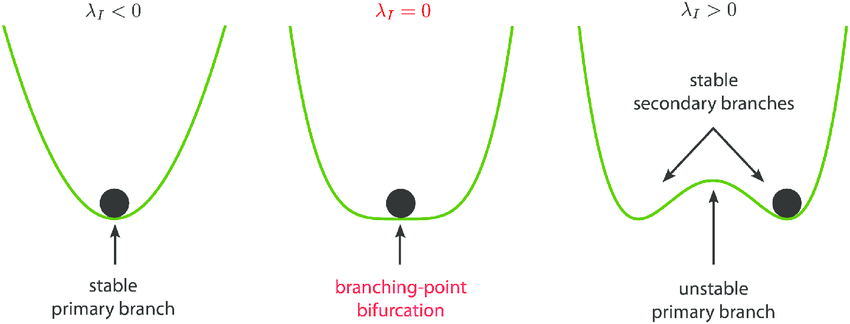
\includegraphics[width=0.75\textwidth]{figures/chapter_SM/SSB}
        \caption{
        A schematic diagram of the Higgs potential~\cite{Potential}.}
        \label{fig:SM}
    \end{center}
\end{figure}

When $\lambda_{1}$ and $\lambda_2$ both take on a negative value, the potential, though symmetric, has a minimum value not found at 0. The minimal value is found instead at $\nu$. At this minimum point of the potential, the vacuum expectation value is:

\begin{equation}
    \phi_{0} = \frac{1}{\sqrt{2}}
    \begin{pmatrix}
        0\\
        \nu
    \end{pmatrix}
\end{equation}

While the overall potential is still symmetric, the particle is no longer at a symmetric equilibrium. The symmetry is ``spontaneously broken". 

It is shown in~\cite{peskin2018introduction} that mass can be obtained when a gauge transformation is performed on the vacuum expectation value:

\begin{equation}
    \phi_{0} = \frac{1}{\sqrt{2}}
    \begin{pmatrix}
        0\\
        \nu+h(x)
    \end{pmatrix}
\end{equation}

where h(x) is the perturbation of the field along the x direction.

This leads to the $D_{\mu} \phi$ in the third to last term~\ref{eq:SMLagrangian} to take the following form:

\begin{equation}
    D_{\mu}\ = (\partial_{\mu}- ig W_{\mu}^{a}\Tau^{a} - i\frac{1}{2}g' B_{\mu}) \phi
\end{equation}

where W and B are weak isospin and weak hypercharge gauge fields defined as above, with g and g' are their corresponding coupling constants. %It can be shown that g and g' are related to each other by the weak mixing angle(also known as the Weinberg angle). 

Plugging this back into the Lagrangian in Equation~\ref{eq:SMLagrangian}, the change in the Lagrangian will become:

\begin{equation}
    \Delta \mathcal{L} = \frac{1}{2} \frac{\nu^{2}}{4}[g^{2}(W^{1}_{\mu})^2 + g^{2}(W_{\mu}^{2})^{2} + (-g W_{\mu}^{3}+ g'B_{\mu})^2]
\end{equation}

With the following substitutions:

\begin{equation}
    W^{\pm}_{\mu} = \frac{1}{\sqrt{2}}(W_{\mu}^{1} \mp iW^{2}_{\mu}) 
\end{equation}

\begin{equation}
    Z^{0}_{\mu}=\frac{1}{\sqrt{g^{2}+g'^{2}}}(g'W_{\mu}^{3} + gB_{\mu})
\end{equation}

\begin{equation}
    \gamma_{\mu} = \frac{1}{\sqrt{g^{2}+g'^{2}}}(g'A^{3}_{\mu} + g B_{\mu})
\end{equation}

where $W^{\pm}_{\mu}$ is the field of the $W^{\pm}$ bosons, Z is the Z boson field and $\gamma$ is the photon field. 

It can be shown that the mass of the $W^{\pm}$ and $Z_{0}$ boson are~\cite{peskin2018introduction}:

\begin{equation}
    m_{W} = g \frac{\nu}{2}
\end{equation}

\begin{equation}
    m_{Z} = \sqrt{g^{2}+ g'^{2}\frac{\nu}{2}}
\end{equation}

The vector field of the photon remains massless~\cite{peskin2018introduction}: 

\begin{equation}
    m_{\gamma}=0
\end{equation}


This mass gaining process follows from the Goldstone's Theorem~\cite{PhysRev.117.648}. It states that for each broken continuous symmetry, a massless scalar boson will appear. After SSB, the $W^{\pm}$ and Z field acquire mass by ``eating" the degree of freedom from the Goldstone boson. These other bosons thereby acquired mass. 

As a consequence, after SSB, the weak isospin and hyper-weak forces $\SUtwo_{L} \times \Uone_{Y}$ become $\Uone_{EM}$. The familiar electric charge can be shown as a combination the weak and hyperweak coupling:

\begin{equation}
    e= \frac{g g'}{\sqrt{g^{2}+g'^{2}}}
\end{equation}

Here, e is the electric charge, and g and g' are the weak isospin and weak hypercharge couplings. 

The electric charge quantum number can be written as:
\begin{equation}
    Q=T_{3}+\frac{1}{2}Y_{W}
\end{equation}
where Q is the electric charge, $T_{3}$ is the third component in the weak isospin from $\SUtwo_{L}$ and $Y_{W}$ is the hypercharge quantum number from the $\Uone_{Y}$ symmetry. 


\begin{table}[!htb]
    \caption{
        The table shows the particle fields of the SM after SSB. Coupling and mass parameters are provided. 
    }
        %The particle content of the SM after the process of
        %electroweak symmetry breaking.
        %Shown for each particle species are the associated electric charge, $Q$,
        %coupling, and mass (approximate).
        %The $y_i$ are the Yukawa coupling (Equation~\ref{eq:higgs_fermion_coupling}),
        %$\alpha_{\text{EM}}$ is the QED coupling constant (`fine structure constant'),
        %$\mathcal{V}$ indicates the parameters of the CKM matrix, and
        %$\alpha_s$ is the QCD coupling constant.
        %The quantities $\lambda$ and $\mu$ are the Higgs self-coupling parameter
        %and mass terms, respectively, appearing in Higgs potential terms (Equation~\ref{eq:higgs_potential}).
    \begin{center}
        \begin{tabularx}{1\textwidth}{m{1em} c c c c }
        \toprule
        \hline
        & Physical Field & Q & Coupling & Mass [GeV] \\
        \hline
        \rotatebox{90}{\hspace{-0.1cm}\textbf{Quarks} } 
            & \makecell{ \quarkU, \quarkC, \quarkT \\ \quarkD, \quarkS, \quarkB} % FIELD
            & \makecell{ $2/3$ \\ $-1/3$ }% Q
            %& \makecell{ $\mathbf{3}$ \\ $\mathbf{3}$ } % SU(3)
            & \makecell{ ($y_i=$) $1\times10^{-5}$, $7\times10^{-3}$, $1$ \\ ($y_i=$) $3\times10^{-5}$, $5\times10^{-4}$, $0.02$ } % Coupling
            & \makecell{ $2\times10^{-3}$, $1.27$, $173$ \\ $4\times10^{-4}$, $0.10$, $4.18$ }\\% Mass
        \rotatebox{90}{\hspace{-0.1cm}\textbf{Leptons} } 
            & \makecell{ \leptonE, \leptonMu, \leptonTau \\ \neutrinoE, \neutrinoMu, \neutrinoTau } % FIELD
            & \makecell{ $-1$ \\ $0$ }% Q
            %& \makecell{ $\mathbf{1}$ \\ $\mathbf{1}$ } % SU(3)
            & \makecell{ ($y_i=$) $3\times10^{-7}$, $6\times10^{-4}$, $0.01$ \\ -- } % Coupling
            & \makecell{ $5\times10^{-4}$, $0.106$, $1.777$ \\ --}\\% Mass
        \midrule
        \rotatebox{90}{\textbf{Bosons} } 
            & \makecell{ \fieldPhoton \\ \fieldZ \\ (\fieldWp, \fieldWm) \\ \fieldG } % FIELD
            & \makecell{ $0$ \\ $0$ \\ $(+1,-1)$ \\ $0$ }% Q
            %& \makecell{ $\mathbf{1}$ \\ $\mathbf{1}$ \\ $\mathbf{1}$ \\ $\mathbf{8}$ } % SU(3)
            & \makecell{ $\alpha_{\text{EM}} \simeq 1/137$ \\ $\sin \theta_{W} \simeq 0.5$ \\ $\mathcal{V}_{\text{CKM}}$ \\ $\alpha_s \simeq 0.1$ } % Coupling
            & \makecell{ $0$ \\ $91.2$ \\ $80.4$ \\  $0$}\\% Mass
        \midrule
        \rotatebox{90}{\textbf{Higgs} } 
            & \makecell{ \fieldH } % FIELD
            & \makecell{ $0$ }% Q
            %& \makecell{ $\mathbf{1}$ } % SU(3)
            & \makecell{ $\lambda$, $\mu$ } % Coupling
            & \makecell{ $125.09$ }\\% Mass
        \hline
        \bottomrule
        \end{tabularx}
    \end{center}
    \label{tab:sm_content_EWSB}
\end{table}
    

The particle fields and their measured properties after spontaneous symmetry breaking are given in Table~\ref{tab:sm_content_EWSB}.

Mass terms the SM particles are recovered after SSB. The complete SM contains seventeen particles along with their anti-particle counterparts. There are two types of particles, the bosons, and the fermions: The bosons are particles that have integer spin and are the force mediator particles, this include photon, W^{\pm}, Z boson, the gluons and the Higgs boson; The fermions are particles that have half spins.
They include the quark and leptons, which are each divided into three generations. Their experimentally measured values can be found in Figure~\ref{fig:SM} and Table~\ref{tab:sm_content_EWSB}.

    \begin{figure}[!htb]
        \begin{center}
            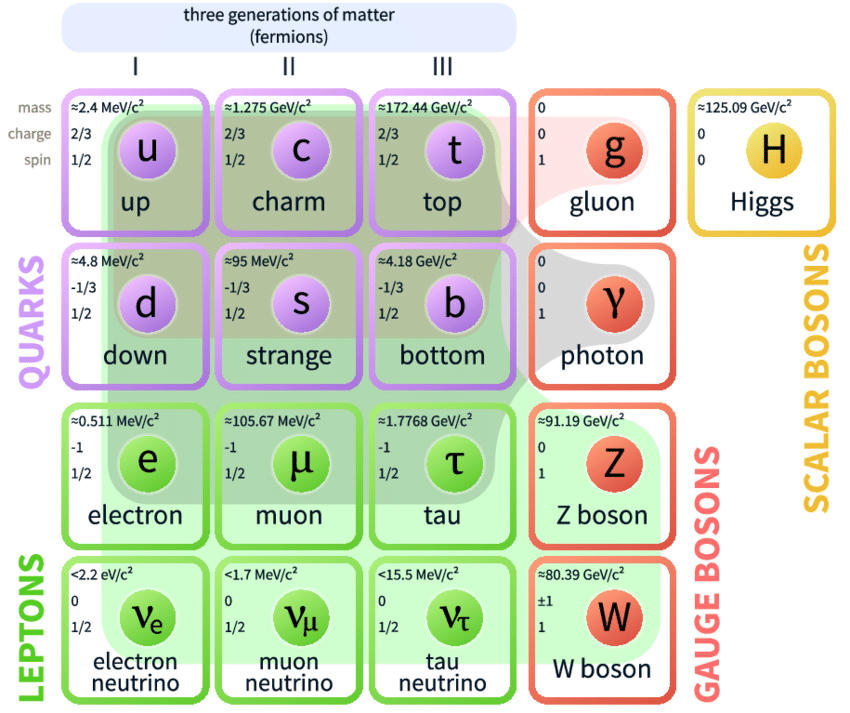
\includegraphics[width=0.75\textwidth]{figures/chapter_SM/SM}
            \caption{
                A schematic diagram of SM particles seen in the scale of the experiment of the Large Hadron Collider ~\cite{enwiki:1060203113}.
            }
            \label{fig:SM}
        \end{center}
    \end{figure}


%\section{Experimental Measurement}
%\label{sec:ExpMeasurement}
%
%
%%Summary plots 
%
%    \begin{figure}[!htb]
%        \begin{center}
%            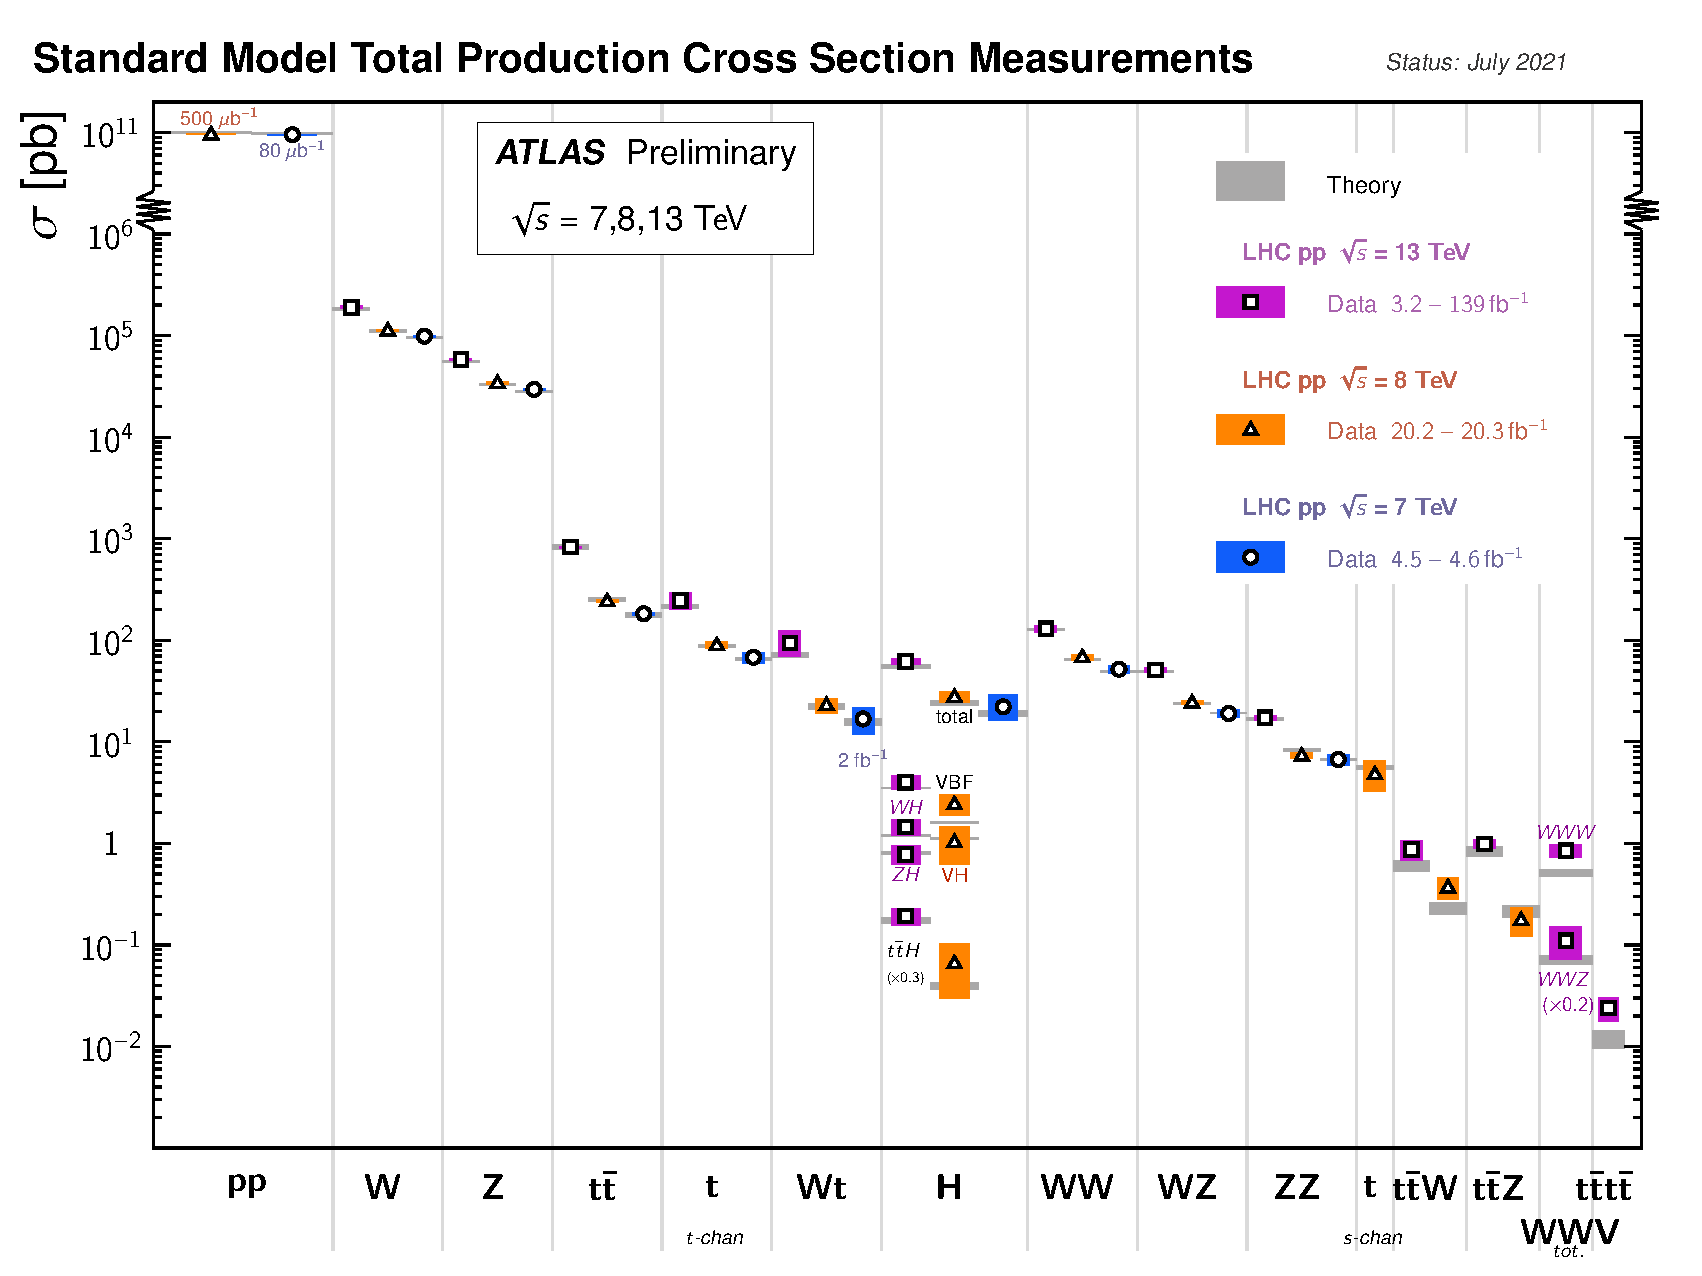
\includegraphics[width=0.75\textwidth]{figures/chapter_SM/SM_Measurement}
%            \caption{
%                A summary plot on the Standard Model cross-section measurements done by the ATLAS experiment~~\cite{ATL-PHYS-PUB-2021-032}.
%            }
%            \label{fig:SM}
%
%        \end{center}
%    \end{figure}
%

%\section{Sucessful Prediction}
%\label{sec:ExpConsistency}
%The Standard Model has many successes in the particle level, and it has made along with many successful predictions, these predictions include:
%    \begin{itemize}
%        \item existence of W boson %~~\cite{}
%        \item existence of Z boson %~~\cite{}
%        \item existence of the charm quark %~~\cite{}
%        \item existence of the top quark %~~\cite{}
%        \item existence of the Higgs boson %~~\cite{}
%    \end{itemize}



\section{Unresolved Problems in the Standard Model}
\label{sec:UnresolvedSM}
The SM in its current form has many standing unresolved problems, and so a more complete theory is out there to be discovered. These proposed extensions to the SM are called Beyond-the-Standard-Model (BSM) theories. The unresolved problems and testing the BSM solutions are the main motivators to many studies done in the particle physics community. In this section, a list of major known existing problems of the SM is summarized.

\subsection{Gravity}
The Standard Model does not include gravity, a fundamental force. Many attempts to reconcile gravity with the existing SM has been made, but it has proven to be challenging. More details can be found in ~\cite{sep-quantum-gravity}.

\subsection{Naturalness}
Naturalness is the property in physics theory where the dimensionless ratio between the free parameters and the physical constants should be of order 1. When a physical theory has a parameter ratio that takes either a very large or small value outside the order of 1, they are considered ``unnatural" and unlikely to be fundamental physics quantities. The Standard Model shows many naturalness issues in different dimensions: in the 0th dimension, there is a cosmological constant problem; in the 2nd order, there is the Higgs Hierarchy problem; lastly, in the fourth dimension, there is the strong CP problem. A detailed description of the problems is laid out in the following.

\subsubsection{The Cosmological Constant Problem}
The Standard Model allows for a 0th dimension constant in its Lagrangian that would not break any of its symmetries. The constant would represent the vacuum energy density and would account for the quantum fluctuation in vacuum. Under Zelokoch's calculations~~\cite{zel1968cosmological}, the relations between the vacuum energy density and the cosmological constant of the Einstein's Equation are directly proportional as such:

\begin{equation}
    \rho_{vac}c^2=\Lambda c^4/8\pi G
\label{eq:cosmoconst}
\end{equation}

Here, $\rho_{vac}$ is the intrinsic density of the vacuum, $\Lambda$ is the cosmological constant, G is the gravitational constant and c is the speed of light. 

The cosmological constant is a well-measured value in cosmology from the measurement of the expansion of the universe. The cutting off in either the Planck scale, a fundamental scale predicted by quantum mechanics or the electro-weak scale in quantum field theory gives a theoretical prediction value of the vacuum expectation value. However, these values do not match. The experimentally measured value of $\rho_{vac}= 5.96 \times 10^{-27} kg/m^{3}$ ~\cite{2016Planck} is about 40-100 order of magnitude smaller than the natural theoretical scale.
This discrepancy poses the biggest naturalness issue in the Standard Model.

%Currently, there are proposition that the discrepany could be due to the fact that the neighboring universe is antropologically different than the whole universe[], or modifications could be done to the Einstein's Equation. But as these propositions violates other universal principle or theorems, none are satisfactory.


%In cosmology, it's known that there is a vacuum energy density that exist in the curvature of the universe that can be expressed as the cosmological constant in the Einstein's Equation. The Cosmological constant is measured with the expansion of the universe and would convert to a vacuum 
%In the 0th order, the cosmological constant as measured by experiment is between 40-100 more order of magniture smaller than predicted. 


\subsubsection{The Higgs Hierarchy Problem}
The Higgs Hierarchy problem describes the apparent large discrepancy in the order of magnitude between the electroweak scale and the gravitational scale, the weak force is about $10^{24}$ greater than gravity. Its effect can be seen in the Higgs boson mass is 17 orders smaller than would be expected by the Planck scale.
A popular solution is quantum corrections via supersymmetry~\cite{2018SUSY}, but as more phasespace for supersymmetry is being ruled out, this solution is increasingly unlikely to solve the problem and is left to be explored by physicists.

\subsubsection{The Strong CP Problem}
\label{sec:strongcp}
The Standard Model allows for a 4-th dimension term that describes strong Charge-Parity(CP) violation naturally:

\begin{equation}
    \mathcal{L}_{QCD} \supset \theta_{QCD}\epsilon_{\mu\nu\rho\sigma} \mathcal{G}^{\mu\nu}\mathcal{G}^{\rho\sigma}
    \label{eq:CPViolation}
\end{equation}

Here, $\mathcal{L}_{QCD}$ is the Lagrangian term of the QCD, $\theta_{QCD}
$ is the parameter that describes CP violation,  $\epsilon_{\mu\nu\rho\sigma}$ is the structure constant. $G^{\mu\nu}G^{\rho\sigma}$ is the strong gauge field.

Experimentally, strong CP violation is not observed: the neutron electric-dipole moment, which is the quantity that measures the positive and negative charge distribution within a neutron, is found to be exceptionally small~\cite{PhysRevLett.124.081803}. As a consequence of the experimental result, the free parameter $\theta_{QCD}$ in Equation ~\ref{eq:CPViolation} is believed to be either exceptionally small or zero. Since, there would be no need for such a term in the theory if the
parameters are exceptionally small, the term's existence in the Lagrangian is therefore seen as ``unnatural". This is known as the strong CP problem.
One well-known solution to the problem is the introduction of the Peccei-Quinn symmetry~\cite{PQSym}. Under this solution, the new field will create a term that naturally cancels with the strong CP term. A particle named ``axion" is predicted by this theory. Many experiments have since been on the lookout for the particle, but it's never yet been observed to date.

\subsection{Neutrino Mass}
The Standard Model does not predict neutrinos to have mass, however, this contradicts experimental findings. Neutrino oscillation, the change of neutrino flavor over time or travel distance, is observed in different solar and reactor experiments. Mathematically, this would only be possible if there must be a mixing angle between the mass eigenstates and flavor eigenstates of neutrinos. This forces the mass of neutrino to be non-zero, contradicting the SM.

Minimally, a minor extension to the SM is required for neutrino mass to be possible in the SM. This is known as the $\nu$-SM theory. Currently, there are two leading camps of $\nu$-SM: the former camp treats neutrinos as a Dirac field, much like other leptons in the SM; the latter predicts neutrinos as a Majorana field, where the anti-neutrinos and the neutrinos is the same particle. Further experiments are required to discover the nature of neutrinos mass. 

%\subsubsection{Triviality Problem}
%Landau pole + asymmototic freedom 


\subsection{Matter-Antimatter Asymmetry}
The Cabibbo-Kobayashi-Maskawa(CKM) matrix of the SM, which descibes how quarks of different types transform from one type to another, allows for some matter-anti matter asymmetry. However, the measured value of the parameter in the SM is not large enough to account for its observed value in the universe. Prediction of matter over antimatter is necessary to account for the observed universe, which includes the formation of galactic structures, stars, and planets. BSM physics will be necessary to account for the asymmetry. 

\subsection{Flavor Problem}
Not all flavors of quarks and leptons are created equal: the mass hierarchy of the quarks and leptons are questions not answered by the SM.

\subsection{Dark Matter and Dark Energy}
SM only accounts for ordinary matter in the universe, which takes up only 4.9\% according to findings from the angular spectroscopy of the cosmic microwave background analysis. It is estimated that dark matter makes about five times as much as ordinary SM particles. However, they are not accounted for in the SM.
Neither is Dark energy, which is estimated to take up 68.3\% of the known content of the universe. Figure~\ref{fig:planck} shows a pie chart that demonstrates the mass-energy distribution of the universe. More details on the diagram and the proposed solution to dark matter in particle form are covered in Chapter~\ref{chapter:DM}.

    \begin{figure}[!htb]
        \begin{center}
            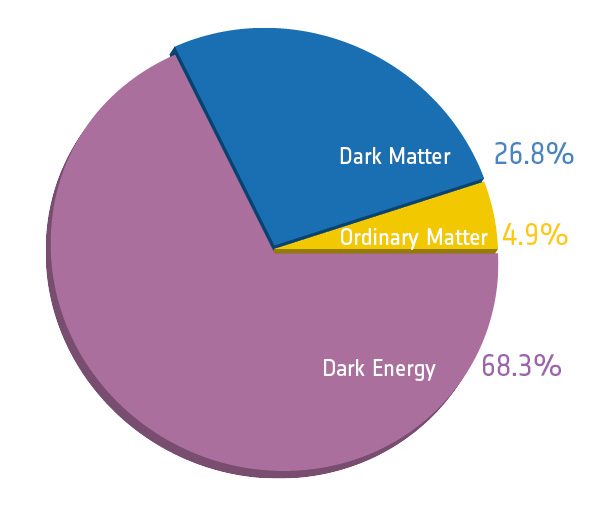
\includegraphics[width=0.75\textwidth]{figures/chapter_SM/Planck}
            \caption{
                The energy distribution of ordinary matter from SM, dark matter and dark energy given from Planck observational data.~\cite{ade2016planck}.
            }
            \label{fig:planck}
        \end{center}
    \end{figure}

\section{Summary}
The SM has led to many breakthroughs in understanding of matter at the fundamental level. Precise measurements of all of the eighteen free SM model parameters~\ref{tab:sm_content_EWSB} are made in different experiments. With the discovery of the Higgs boson in 2012, all the particles predicted by the model are found. However, there remains many open questions left to be solved. These all hints at the existence of a more complete theory beyond what is known. In the next chapter, the SM extension on dark matter will be discussed in detail. 


%As a major motivator to the studies done in this thesis, evidence and hypotheses of dark matter will be examined in length in the next chapter. 

%\section{history}
    %Though the advancement in electrodynamics through the Maxwell's Equations and the progress of Special Relativity, Quantum Theory was re-development with the second quantization\footnote{} , path intergral through the study of Fock, Feynman and Paul Dirac, later led to the development of the quantum field theory.   
    %Paradigm of Quantum field theory, and is the basis where consequent theories in the standard model is based on. 

    %History that lead to the standard model
    %What is the standard model 
%\section{Symmetries}

%1. Electro-Weak theory
%    Q.E.D.
%    Dirac and the problem of annihilation of anti-particle lead to the second quantization, with work from 
%    Gauge theory
%    The unification of eletro-dynamic force and the weak force
%    The Higgs Mechanism / spontaneous symmetry breaking 
%
%4. Quantum Chromodynamics
%    Yang-Mill theory, non-abelian gauge groups. 
%5. Spontaneous Symmetry Breaking 

%-cannot describe atom level in QCD

    %* historically, how it was developed
    %* its sucesses, its predictions lead to W,Z, Higgs boson
    %* Neutrino oscillation or their non-zero mass

%Standard model is the corner stone and a starting point in the journey to particle discoveries, 
